\documentclass[a0,portrait]{a0poster}
\usepackage{multicol}\columnsep=50pt
\usepackage[svgnames]{xcolor}
\usepackage{graphicx}
\usepackage[font=Large,labelfont=bf]{caption}
\usepackage{titlesec}
\usepackage{enumitem}
\usepackage{hyperref}
\hypersetup{
    colorlinks=true,
    linkcolor=blue,
    filecolor=magenta,      
    urlcolor=cyan,
}
\titleformat*{\section}{\huge\bfseries}
\titleformat*{\subsection}{\LARGE\bfseries}

\begin{document}

% Header split into two parts
\begin{minipage}[b]{0.7\linewidth}
\VeryHuge
\textbf{Utilizing Feelings Towards Groups \\ for Improved Voting Predictions} \\[0.5cm]
\huge
\color{Magenta}
\textbf{Aurora Siegel}
\color{Black}
\end{minipage}
\begin{minipage}[b]{0.3\linewidth}
  
\includegraphics[width=20cm]{queens_college.png}
\end{minipage}
\vspace{0.5cm}

% Body with it's default font size
\begin{multicols}{2} 
\Large

\vspace{-1cm}
\section*{Hypothesis}

Voter feelings towards newer and hot-button issue-related groups in the media are more predictive of voting behavior than feelings towards long-standing groups such as race and religion.

\vspace{-1cm}
\section*{Methodology}

The Democracy Fund Voter Study Group \cite{dfvsg} report of 5,642 representative voters was investigated. Limitations of this dataset include:

\begin{itemize}[leftmargin=2cm]
\item[--] No age demographic information.
\item[--] Representation issues to the survey being conducted online.
\item[--] Trust respondents to accurately report the candidate they voted.
\end{itemize}

\noindent
Analysis was done using a Logistic Regression on $[0,1]$ normalized variables. Performance was measured over a 10-fold train/test split. All models included party and demographic control variables. To verify the strength of feeling thermometer variables we also included important issue variables in some models.

\subsection*{Dependent Variable - Clinton}

The goal is to predict which 2016 U.S. presidential candidate a voter would vote for. The 5,642 voters who reported voting for either Trump or Clinton, encoded as 0 and 1 respectively, were used.

\subsection*{Independent Variables - Feeling Thermometer}

This study's independent variables were measured through a feelings thermometer that scaled from 0 (very cold or unfavorable feeling) to 100 (very warm or favorable feeling).

\begin{center}
  \begin{tabular}{|cc|cc|} \hline
    \multicolumn{2}{|c|}{\color{DarkMagenta}Race/Religion Group Identities} & \multicolumn{2}{|c|}{\color{CornflowerBlue}Hot-Button Group Identities} \\ \hline
    Black & Christian & Wall St. & Immigrant \\
    White & Muslim &  Union & Black Lives Matter \\
    Hispanic & Jew & Gays & Alt-Right \\
    Asian & & Police & Feminist \\
    \hline
  \end{tabular}
\end{center}

\begin{center}
  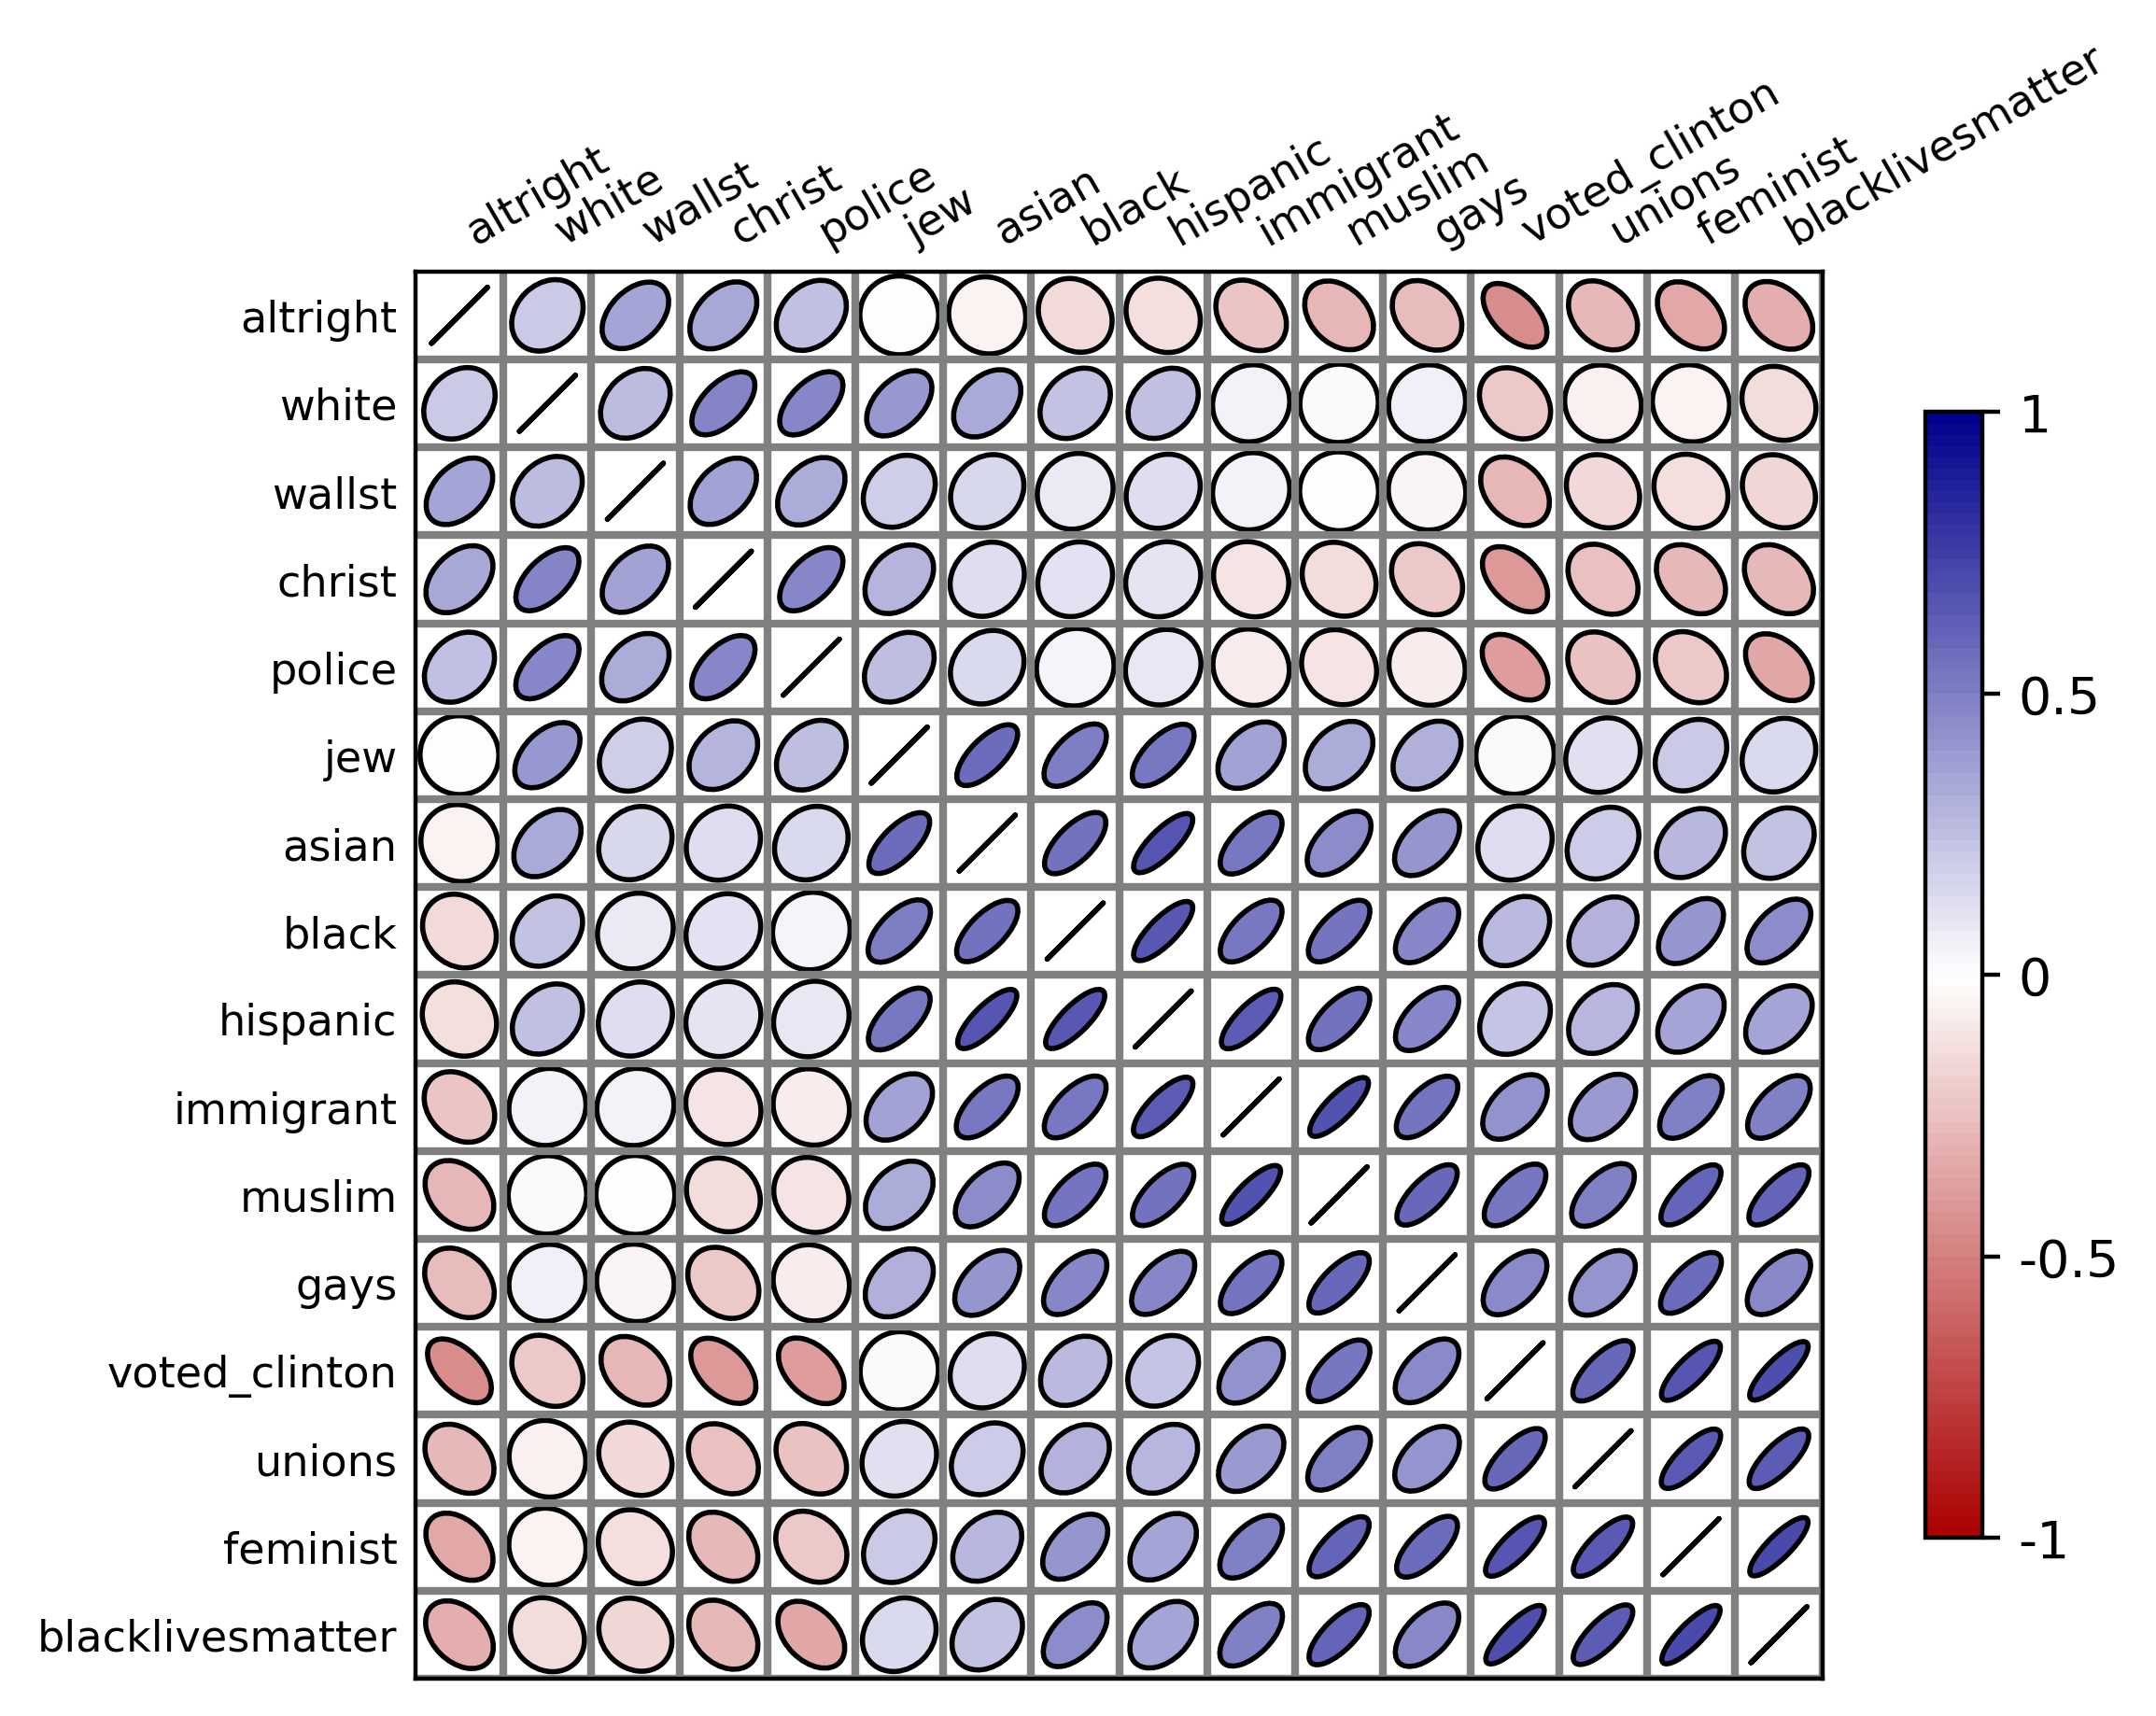
\includegraphics[width=1.0\linewidth]{correlation_all.png}
  \captionof{figure}{Variable Correlation}
  \label{fig:AllCorrelation}
\end{center}

\vspace{-1cm}
\section*{Results}
\vspace{-1cm}
\begin{center}
  {\renewcommand{\arraystretch}{1.2}
  \begin{tabular}{|l|c|c|} \hline
    \textbf{Model} & \textbf{Mean Accuracy} & \textbf{Mean Accuracy (Issue)} \\ \hline
    No Feeling Thermometer & 80.47\% & 90.95\% \\ \hline
    {\color{DarkMagenta}Race/Religion} & 87.83\% & 91.38\% \\ \hline
    {\color{CornflowerBlue}Hot-Button} & 91.90\% & 93.02\% \\ \hline
  \end{tabular}}
  \captionof{figure}{Performance 10-fold Logistic Regression models. T-test reports a p-value of 0.041 that the Hot-Button with Issue model is better than the respective Race/Religion model.}
  \label{fig:scores}
\end{center}

\begin{center}
  {\renewcommand{\arraystretch}{1.1}
\begin{tabular}{|l|r|r|} \hline
\textbf{Variable} & \textbf{Coefficient} & \textbf{P-value} \\ \hline \hline
Constant & 0.9889 & 0.099 \\ \hline
{\color{DarkMagenta}Feelings towards black} & -1.1753 & \textbf{0.003} \\ \hline
{\color{DarkMagenta}Feelings towards white} & 0.1589 & 0.705 \\ \hline
{\color{DarkMagenta}Feelings towards hispanic} & -0.4972 & 0.213 \\ \hline
{\color{DarkMagenta}Feelings towards asian} & -0.4818 & 0.233 \\ \hline
{\color{DarkMagenta}Feelings towards christ} & -0.84 & 0.015 \\ \hline
{\color{DarkMagenta}Feelings towards muslim} & 1.8646 & \textbf{0.000} \\ \hline
{\color{DarkMagenta}Feelings towards jew} & -0.1891 & 0.634 \\ \hline
{\color{CornflowerBlue}Feelings towards gays} & 0.1523 & 0.636 \\ \hline
{\color{CornflowerBlue}Feelings towards immigrant} & 1.1409 & \textbf{0.001} \\ \hline
{\color{CornflowerBlue}Feelings towards feminist} & 2.4349 & \textbf{0.000} \\ \hline
{\color{CornflowerBlue}Feelings towards black lives matter} & 2.2431 & \textbf{0.000} \\ \hline
{\color{CornflowerBlue}Feelings towards wallst} & -1.9854 & \textbf{0.000} \\ \hline
{\color{CornflowerBlue}Feelings towards unions} & 1.508 & \textbf{0.000} \\ \hline
{\color{CornflowerBlue}Feelings towards police} & -1.1085 & \textbf{0.001} \\ \hline
{\color{CornflowerBlue}Feelings towards alt-right} & -2.7727 &  \textbf{0.000} \\ \hline
Demographic education & 0.3554 & 0.135 \\ \hline
Demographic male & -0.0533 & 0.680 \\ \hline
Demographic income & 0.5391 & 0.030 \\ \hline
Demographic white & 0.1225 & 0.693 \\ \hline
Demographic black & 1.5446 & \textbf{0.000} \\ \hline
Demographic asian & 0.7029 & 0.191 \\ \hline
Demographic hispanic & 0.7258 & 0.068 \\ \hline
Aligns democrat & 1.5772 & \textbf{0.000} \\ \hline
Aligns republican & -1.3828 & \textbf{0.000} \\ \hline
Is important crime & 0.3319 & 0.415 \\ \hline
Is important economy & 1.2859 &  \textbf{0.006} \\ \hline
Is important immigration & -1.9346 & \textbf{0.000} \\ \hline
Is important religious liberty & -1.2238 & \textbf{0.000} \\ \hline
Is important terrorism & -1.7389 & \textbf{0.000} \\ \hline
Is important gay rights & 0.7859 & \textbf{0.002} \\ \hline
Is important money in politics & 0.1385 & 0.551 \\ \hline
Is important jobs & -0.9182 & 0.011 \\ \hline
Is important taxes & -1.1551 &  \textbf{0.001} \\ \hline
Is important abortion & -0.1409 & 0.496 \\ \hline
Is important racial equality & 1.2266 & \textbf{0.000} \\ \hline
Is important gender equality & 1.5613 & \textbf{0.000} \\ \hline
\end{tabular}}
  \captionof{figure}{Logistic Regression input variables when run on all respondents and with all variables included. Significance to the $99^{th}$ percentile is bolded.}
  \label{fig:coefficients}
\end{center}

\vspace{-1cm}
\section*{Conclusion}

\noindent
Voter opinions on long-term identities (race and religion) are less predictive of voting behavior than their opinions on more recent hot-button groups.

\vspace{0.5cm}
\noindent
Future work can investigate whether asking about trending topics will mollify the Bradley Effect. Voters might be more willing to divulge opinions if they are not feeling judged. 

\vspace{0.5cm}
\noindent
Pursuing the strong predictive power of variables like Feelings towards Black Lives Matter (88.2\%) over including both Feelings towards Blacks and Feelings towards Police together (83.7\%) can also be worthwhile.

\begin{thebibliography}{9}
\bibitem{dfvsg}
\textit{Democracy Fund Voter Study Group 2016} data retrieved from \url{https://www.voterstudygroup.org/publication/2016-voter-survey}
\end{thebibliography}

\vspace{0.5cm}
\noindent
This work was made possible through the advice and guidance offered by Dr. Ryan Sperry and Karol Zieba. Code to reproduce this poster can be found at \url{https://github.com/aurorasiegel/feelings}

\end{multicols}
\end{document}
